\chapter{Radiation Effects on Electronics}
\label{sec:radiation_effects}

To design electronic circuits for accelerator applications, it is essential to understand the basic effects of radiation on electronic components. Radiation is not unique to CERN; it exists naturally on Earth and throughout the Solar System, and it is also produced artificially for medical applications, scientific experiments, and energy production. However, different environments involve different radiation fields, depending on the particles present. This chapter provides an overview of particle interactions with matter and the resulting effects on electronics. Finally, it briefly introduces the radiation environment of the LHC and the facilities used for testing.

\section{Particles Interaction with Matter}
\label{section:particles-matter-interaction}

\subsection{Photons}
\label{subsection:photons}
Photons are neutral, massless elementary particles that serve as the quanta of electromagnetic fields. Thus, they can only travel at the speed of light in a vacuum but they still carry both energy and momentum.

\begin{figure}[H]
    \centering
    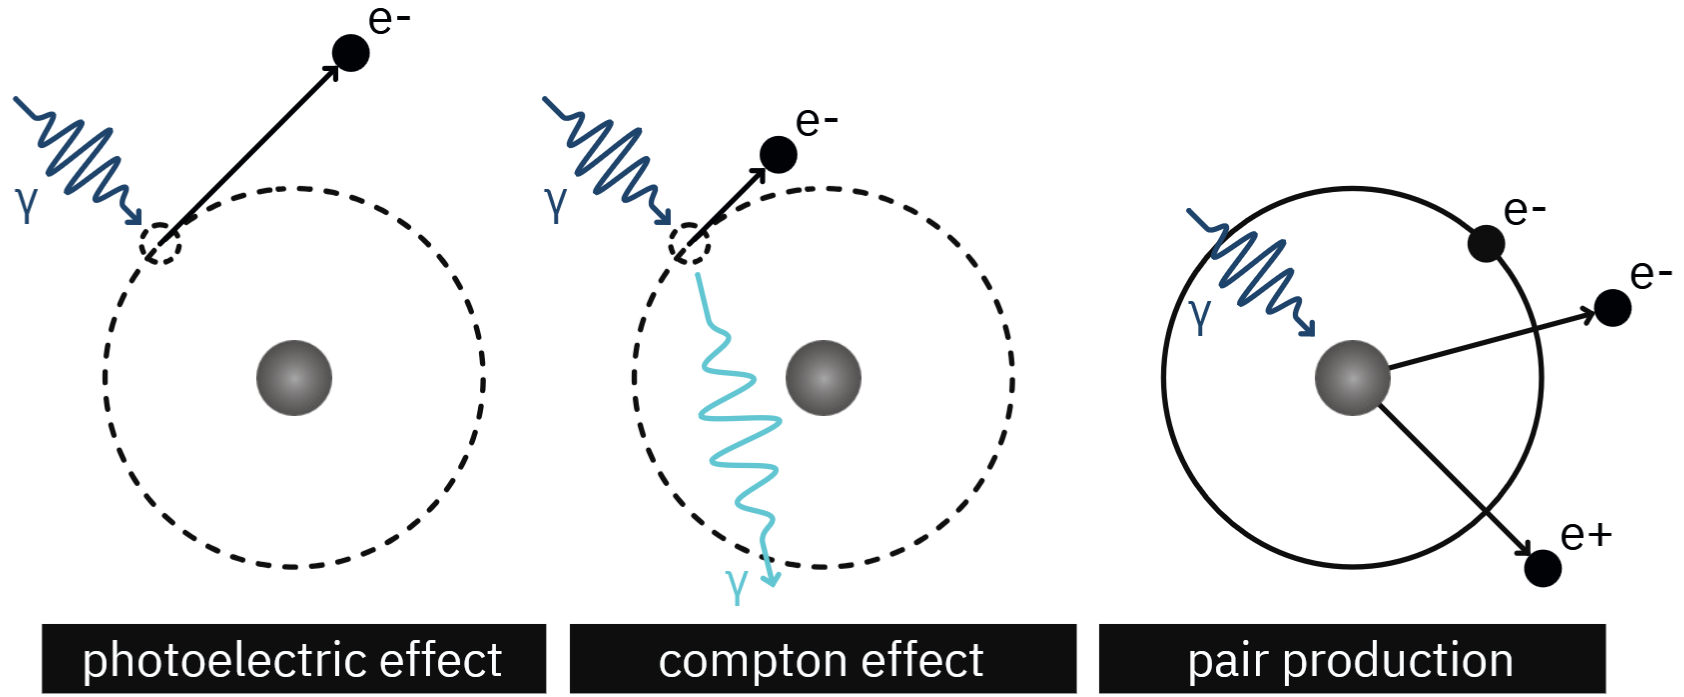
\includegraphics[width=0.7\linewidth]{02_RadiationEffectsOnElectronics/images/photons.png}
    \caption{Representation of the different photon--matter interaction mechanisms. Image taken from~\cite{jung_2023_thesis}.}
    \label{fig:photon-interactions}
\end{figure}

\textbf{Rayleigh scattering} is the process in which a photon is scattered by atomic electrons without transferring energy to them. Therefore, the photon keeps approximately the same energy, while only its direction changes.

\textbf{The photoelectric effect} occurs when the photon energy is close to or higher than the binding energy of an electron. In this case, the photon is absorbed and transfers all of its energy to the electron, which is ejected from the atom.

\textbf{Compton scattering} occurs when the photon energy is much larger than the binding energy of the electron. The photon transfers part of its energy to the electron and is scattered with lower energy. The electron receives enough energy to be ejected from its orbit.

\textbf{Pair production} occurs when a photon passes close to the nucleus of an atom and its energy is above the threshold $E_\gamma \geq 2m_ec^2$, where $m_e$ is the electron mass. In this case, the photon can be converted into an electron--positron pair.

\subsection{Charged Particles and Neutrons}
\label{subsection:charged-particles-neutrons}

Two types of particles are discussed below: charged particles and neutrons. Unlike charged particles, neutrons are electrically neutral. Therefore, they interact with matter primarily through \textbf{nuclear interactions}, as they do not experience the Coulomb force that dominates the energy-loss mechanisms of charged particles~\cite{cas_borovets_2025}. Charged particles, on the other hand, undergo both \textbf{Coulombic} and nuclear interactions.

In the following discussion, the term charged particles refers to particles such as protons ($p^+$), charged pions ($\pi^\pm$), charged kaons ($K^\pm$), electrons ($e^-$), and positrons ($e^+$). These particles may carry either a positive or a negative electric charge. The positron, $e^+$, is the positively charged antiparticle of the electron, $e^-$.

\subsubsection*{Nuclear Interactions}

\begin{figure}[H]
    \centering
    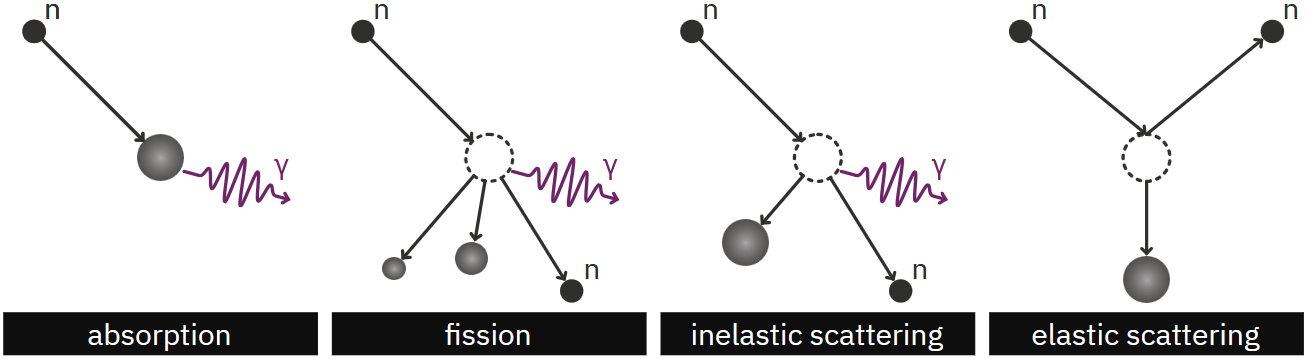
\includegraphics[width=0.95\linewidth]{02_RadiationEffectsOnElectronics/images/neutrons.png}
    \caption{Representation of the different nuclear interactions. Image taken from~\cite{jung_2023_thesis}.}
    \label{fig:nuclear-interactions}
\end{figure}

\textbf{Radiative capture} is a neutron-absorption reaction in which the incident neutron is captured by a nucleus, forming an excited compound nucleus. The nucleus subsequently de-excites by emitting one or more gamma rays. Radiative capture is particularly important for slow and thermal neutrons, whose average kinetic energy at room temperature is approximately \SI{0.025}{\electronvolt}, although its probability depends strongly on the target nucleus~\cite{knoll_2010_ch2}.

\textbf{Fission} occurs when a heavy nucleus splits into two or more lighter nuclei, known as fission fragments, usually after absorbing a neutron. The reaction releases a large amount of energy and is generally accompanied by the emission of secondary neutrons and gamma rays. The probability of neutron-induced fission depends strongly on both the target isotope and the neutron energy; therefore, no universal threshold such as \SI{20}{\mega\electronvolt} can be assigned~\cite{knoll_2010_ch2}.

\textbf{Inelastic scattering} occurs when an incident neutron or charged hadron transfers part of its kinetic energy to a nucleus, leaving the nucleus in an excited state. The outgoing particle therefore has lower kinetic energy. The excited nucleus subsequently de-excites, commonly through gamma-ray emission. Inelastic scattering generally requires the incident particle to have sufficient energy to excite a nuclear state~\cite{knoll_2010_ch2}.

\textbf{Elastic scattering} occurs when an incident neutron or charged particle collides with a nucleus and is deflected, causing the nucleus to recoil. The projectile and nucleus remain internally unchanged, and the total kinetic energy of the system is conserved. For neutrons, elastic scattering is particularly important for moderation, since repeated collisions reduce the neutron energy until thermal equilibrium with the surrounding material is approached~\cite{knoll_2010_ch2}.

\subsubsection*{Coulomb Interactions}

Coulomb interactions describe the interactions of charged particles with the electric fields of atomic electrons and nuclei. Unlike neutrons, charged particles lose a substantial part of their energy through these electromagnetic interactions. Charged hadrons may additionally undergo nuclear interactions.

\begin{figure}[H]
    \centering
    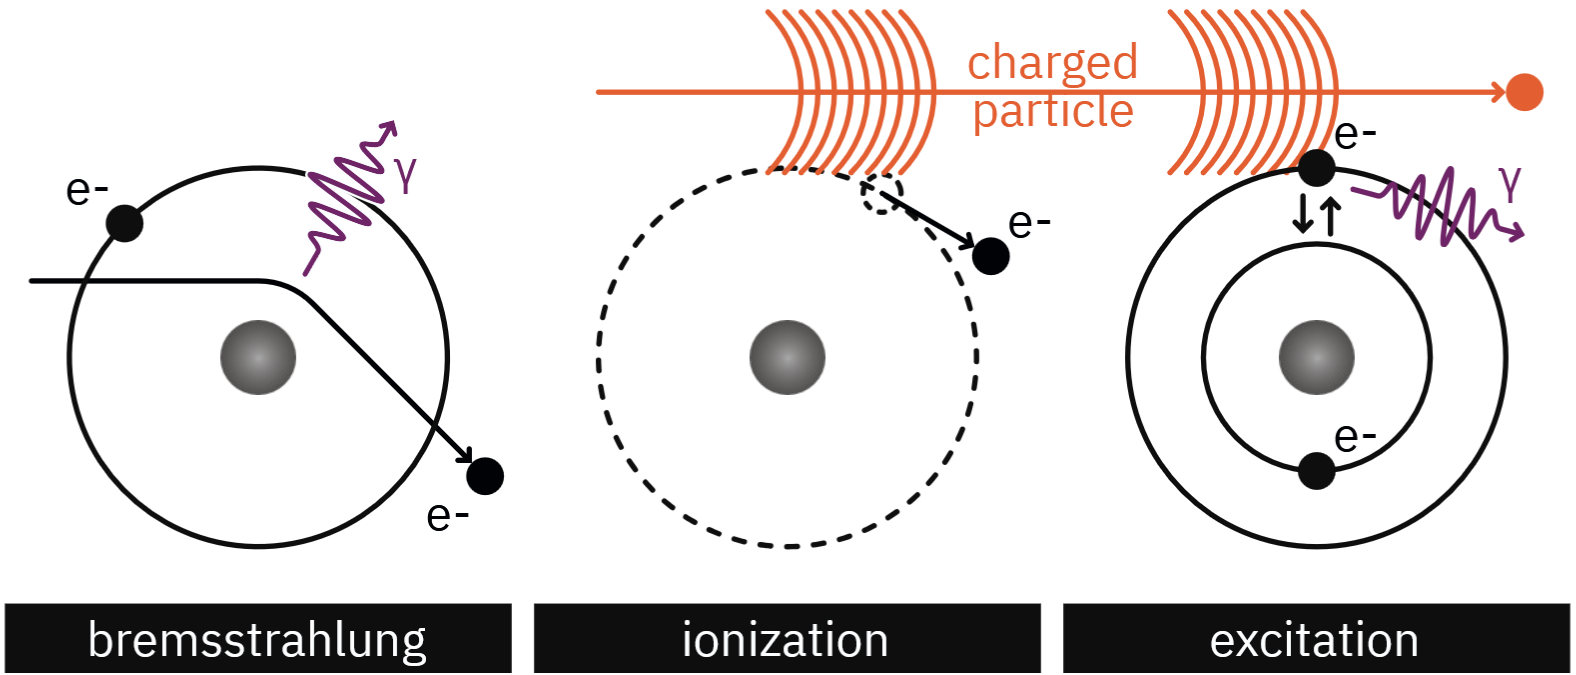
\includegraphics[width=0.7\linewidth]{02_RadiationEffectsOnElectronics/images/charged-particles.png}
    \caption{Schematic representation of the principal Coulomb interaction mechanisms of charged particles with matter. Image adapted from~\cite{jung_2023_thesis}.}
    \label{fig:coulombic-interactions}
\end{figure}

\textbf{Bremsstrahlung} occurs when a charged particle is deflected or decelerated by the electric field of an atomic nucleus. As a result, part of the particle's kinetic energy is emitted as a photon. Although this process can occur for any charged particle, it is particularly significant for light particles, especially electrons and positrons.

\textbf{Ionization} occurs when a charged particle transfers sufficient energy to a bound atomic electron to eject it from the atom. This process leaves behind a positively charged ion and produces a free electron. In semiconductor materials, the deposited energy can generate electron--hole pairs.

\textbf{Excitation} occurs when a charged particle transfers energy to a bound electron without ejecting it from the atom. The electron is promoted to a higher bound energy state. When it returns to a lower energy state, the excess energy may be released through photon emission.

For charged particles mainly interact through Coulomb forces and thereby only a small fraction of energy is used for nuclear reactions, and thus ionizing dose effects are dominant for them~\cite{barbottin1999instabilities}.

\subsection{Energy Transfer In Matter}
\label{subsection:energy-transfer}

As showcased in Subsection~\ref{subsection:charged-particles-neutrons}, when a particle penetrates a material, it gradually transfers its energy to matter both by the direct ionization which occurs from the primary interactions and with the indirect between the generated particles, namely secondary particles, and matter. The impinging particle is expected to experience an energy loss, which can be divided in \textit{i) Ionizing Energy Loss (IEL)} and \textit{ii) Non-Ionizing Energy Loss (NIEL)}.

To quantify the deposition of energy to matter, the concept of Linear Energy Transfer (LET) is introduced in Equation~\ref{eq:let}, and expressed in \si{\kilo\electronvolt\per\micro\metre}.

\begin{equation}
    LET = \frac{\mathrm{d}E}{\mathrm{d}x}
    \label{eq:let}
\end{equation}

For a charged particle with kinetic energy $E$, the stopping power is defined as~\cite{knoll_2010_ch2}

\begin{equation}
    S = - \frac{\mathrm{d}E}{\mathrm{d}x}
    \label{eq:stopping-power}
\end{equation}

and shows the rate at which the particle is losing its energy with respect to the distance it travels. The negative sign ensures that the stopping power is positive, since the kinetic energy of the particle decreases as it propagates through the material. Taking into consideration the material and its corresponding density, the \textbf{mass stopping power} is defined as

\begin{equation}
    S_m = - \frac{1}{\rho} \cdot \frac{\mathrm{d}E}{\mathrm{d}x}
    \label{eq:mass-stopping-power}
\end{equation}

and is commonly expressed in \si{\mega\electronvolt\centi\metre\squared\per\gram}.

Going back to the definitions of IEL and NIEL, the total stopping power can be approximated as the superposition of the two.

\begin{equation}
    S_{total} = S_{IEL} + S_{NIEL} = - \left[ \left( \frac{dE}{dx} \right)_{IEL} + \left( \frac{dE}{dx} \right)_{NIEL} \right]
    \label{eq:stopping-power-total}
\end{equation}

and the corresponding total mass stopping power

\begin{equation}
    S_{m,total} = \frac{1}{\rho} S_{total} =  - \frac{1}{\rho} \cdot \left[ \left( \frac{dE}{dx} \right)_{IEL} + \left( \frac{dE}{dx} \right)_{NIEL} \right]
    \label{eq:mass-stopping-power-total}
\end{equation}

\textbf{IEL} refers to the energy transferred mainly to atomic electrons, thereby causing ionization and excitation. The accumulation of this ionizing energy deposition is responsible for Total Ionizing Dose (TID). On the other hand, \textbf{NIEL} refers to the energy transferred to atomic nuclei, which can displace atoms from their lattice positions and create defects in the material. It is therefore associated with Displacement Damage (DD), which can be expressed through the Displacement Damage Dose (DDD) or the Total Non-Ionizing Dose (TNID).

For charged particles, IEL is generally the dominant energy-loss mechanism, although the contribution of IEL and NIEL depends on the particle type and its energy. Neutrons do not directly cause significant ionization because they do not carry an electric charge. However, their interactions with atomic nuclei can generate recoil nuclei and secondary charged particles, which may then cause both ionization and displacement damage.

Single-Event Effects (SEE) do not constitute another type of stopping power. Instead, they are effects caused by a single particle interaction inside a sensitive region of an electronic device.

\section{Radiation Effects on Electronics}
\label{section:radiation-effects-electronics}

\subsection{Total Ionizing Dose (TID}
\label{subsection:tid}

TID results from the cumulative ionizing energy deposited in a material. Its SI unit is the gray (\si{\gray}), where \SI{1}{\gray} corresponds to \SI{1}{\joule\per\kilogram} of absorbed energy. Equation~\ref{eq:tid-calculation} describes the calculation of TID using the conversion factor $K_{\mathrm{Gy}} = 1.602\times10^{-7},\si{\gray\milli\gram\per\mega\electronvolt}$, the particles fluence $\Phi$ in \si{\centi\metre\squared} and $p$ represents the different types of particles that are present in the LHC environment.

\begin{equation}
    \mathrm{TID}^\pm
    =
    \sum_{p=e^{\pm},\,\pi^{\pm},\,p^{\pm},\,K^{\pm},\,\mu^{\pm}}
    \int_{0}^{E_{\max}}
    K_{\mathrm{Gy}}
    \cdot
    \frac{\mathrm{LET}(E,p)}{\rho}
    \cdot
    \Phi(E,p)
    \,\mathrm{d}E
    \label{eq:tid-calculation}
\end{equation}

Photons do not lose energy continuously through Coulomb interactions. Instead, they transfer energy through processes, such as the photoelectric effect, Compton scattering, and pair production. Their TID contribution is therefore calculated using the mass energy-absorption coefficient $\mu_{\mathrm{en}}(E)/\rho$, expressed in \si{\square\centi\metre\per\gram}.

For a monoenergetic photon fluence $\Phi_{\gamma}(E_0)$ at energy $E_0$, the corresponding TID contribution is

\begin{equation}
    \mathrm{TID}^{\gamma}(E_0) = K_{\mathrm{Gy}} \frac{\mu_{\mathrm{en}}(E_0)}{\rho} E_0 \Phi_{\gamma}(E_0)
    \label{eq:monoenergetic-photon-tid} 
\end{equation}

Therefore, for a continuous photon energy spectrum, the contributions from all photon energies are integrated as

\begin{equation} 
    \mathrm{TID}^{\gamma} = K_{\mathrm{Gy}} \int_{0}^{E_{\max}} \frac{\mu_{\mathrm{en}}(E)}{\rho} E \phi_{\gamma}(E) \,\mathrm{d}E, 
    \label{eq:photon-tid} 
\end{equation}

where $\phi_{\gamma}(E)=\mathrm{d}\Phi_{\gamma}/\mathrm{d}E$ is the differential photon fluence spectrum.

Therefore, the total TID in a mixed-field environment is given by the sum of the charged-particle and photon contributions: 

\begin{equation} 
    \mathrm{TID} = \mathrm{TID}^{\pm} + \mathrm{TID}^{\gamma} 
    \label{eq:total-tid} 
\end{equation}

\subsection{Displacement Damage Dose (DDD)}
\label{subsection:dd}

Displacement damage occurs via Coulombic or nuclear scattering and is attributed to NIEL. An impinging particle can displace a nucleus in the material lattice, thus creating defects in the structure of the semiconductor for example, and is calculated similarly to the TID but using the NIEL and normalizing with mass density and multiplied by particle fluence as expressed in Equation~\ref{eq:ddd}.

\begin{equation}
    \mathrm{DDD} = \frac{NIEL}{\rho} \cdot \Phi
    \label{eq:ddd}
\end{equation}

As shown in Figure~\ref{fig:displacement-damage}, these atomic displacements that break the regularity of the crystal lattice, create vacancies (missing atoms), interstitial (atom placed in a non-lattice position) and even a combination of these which is called a Frenkel pair.

\begin{figure}[H]
    \centering
    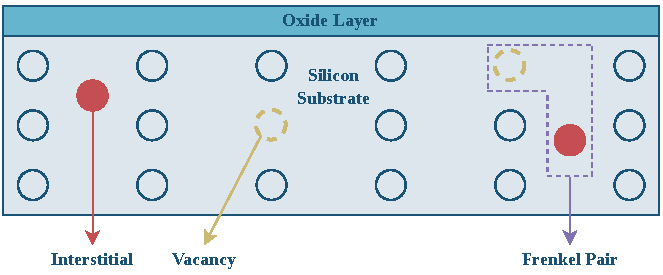
\includegraphics[width=0.85\linewidth]{02_RadiationEffectsOnElectronics/images/dd_effects.pdf}
    \caption{Primary lattice defects induced by displacement damage in silicon.}
    \label{fig:displacement-damage}
\end{figure}

However, it is a very complex task to predict the long term DDD for complex real-world radiation environment, such the mixed field of CERN. While several units exist to represent displacement damage, in the scope of the thesis, the Displacement Damage Equavalent Fleunce (DDEF) is used to normalize the entire environment into an equivalent, single-energy particle fluence. More specifically, the 1 MeV neutron equivalent fluence is used as it is the standard metric at CERN, and corresponds to the amount of 1 mEV neutron fluence necessary to induce an equivalent to the fluence of the considered particle in the material~\cite{ASTME722_2014}. 

\begin{equation}
DDEF = \Phi_{1\text{MeV } neq.} = \kappa_{n_{1\text{MeV}}}(E) \cdot \Phi(E) = \frac{NIEL(E)}{NIEL(n_{1\text{MeV}})} \cdot \Phi(E)
\end{equation}

Here, $\kappa_{n_{1\text{MeV}}}$ is the hardness parameter, obtained by dividing the NIEL of the particle by the NIEL of the 1 MeV neutron. The overall DDEF in a radiation environment can be obtained by summing the contributions of all particles:

\begin{equation}
DDEF = \sum_{p} \int k(p,E) \cdot \Phi(p,E) \cdot dE
\end{equation}

\subsection{Single Event Effects (SEE)}
\label{subsection:see}

In contrast to cumulative damage mechanisms, a Single Event Effect (SEE) is a stochastic phenomenon triggered by the interaction of a single energetic particle with the semiconductor material. Therefore, for the analysis of radiation test data, it is critical to note that SEEs do not depend on the Total Ionizing Dose (TID) or the Displacement Damage Dose (DDD), but are instead explicitly attributed to particle fluence and flux. 

Particle flux, $\varphi$, represents the rate at which particles pass through a unit area per unit time, defined as:
\begin{equation}
    \varphi = \frac{d\Phi}{dt} = \frac{1}{A} \frac{dN}{dt}
\end{equation}
where $N$ is the number of particles and $A$ is the cross-sectional area. Flux is typically measured in units of $\text{cm}^{-2}\cdot\text{s}^{-1}$. Consequently, a higher particle flux directly translates to a higher rate of SEE occurrences over time.

Integrating the flux over a specific time interval yields the particle fluence, $\Phi$, which is the total number of particles that have impinged on a unit area ($\text{cm}^{-2}$):

\begin{equation}
    \Phi = \int \varphi \, dt = \frac{N}{A}
\end{equation}

A higher total fluence inherently increases the statistical probability of an SEE occurring during the device's operational lifetime.

For the scope of this thesis, the primary metric used to evaluate system robustness against SEEs is the device cross-section ($\sigma$). The cross-section quantifies the sensitivity of the component to a specific radiation environment and represents an effective operational "target area" for a given type of event. It is defined as the number of recorded single event effects divided by the total particle fluence:
\begin{equation}
    \sigma = \frac{N_{\text{events}}}{\Phi}
\end{equation}
The cross-section $\sigma$ is conventionally expressed in units of $\text{cm}^2$ per device (or per bit for memory structures).

\subsubsection*{Effects on Semiconductors}

When a high-energy particle passes through a semiconductor, it punches through the material and leaves behind a dense trail of electrical charges (electron-hole pairs). As shown in Figure~\ref{fig:see-semiconductors}, the internal electric field of the transistor quickly pulls these charges apart, temporarily warping the local field into a funnel shape. This sudden movement creates a sharp, rapid spike of electrical current ($I_{\text{drift}}$), which is followed by a slower, lingering current ($I_{\text{diff}}$) as leftover charges drift back toward the transistor node. Every digital circuit has a specific threshold called the critical charge ($Q_{\text{CRIT}}$), which is the minimum amount of electrical charge required to flip a digital state. If the combined current spike deposits a total charge that exceeds $Q_{\text{CRIT}}$, a bit-flip or data glitch occurs. Modern microchips are highly vulnerable to this because smaller transistors require much less charge to flip, and they are packed so tightly together that a single particle can easily corrupt multiple adjacent transistors at the same time.

\begin{figure}[H]
    \centering
    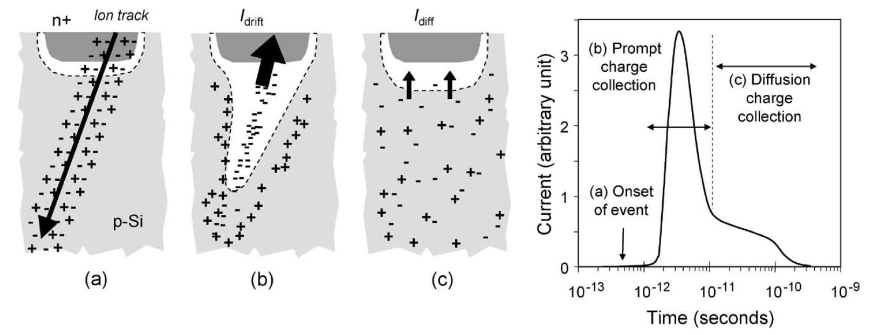
\includegraphics[width=\textwidth]{02_RadiationEffectsOnElectronics/images/see-semiconductor.png}
    \caption{Mechanism of charge collection causing SEEs in a semiconductor junction, adapted from~\cite{bricas_2022_thesis}.}
    \label{fig:see-semiconductors}
\end{figure}

\subsubsection*{Non-Destructive (Soft) Types of SEE}

\textbf{Single-Event Upset (SEU)} occurs when an incident particle causes a non-destructive state change (a bit-flip from 1 to 0 or vice versa) in a latched logic or memory cell. The element remains fully functional and can be recovered by a rewrite or reset operation~\cite{aguiar_see_nondestructive_2024}.

\textbf{Single-Event Transient (SET)} occurs when a single energetic particle strike induces a temporary voltage excursion or spike at a node within an integrated circuit~\cite{aguiar_see_nondestructive_2024}.

\textbf{Single-Event Functional Interrupt (SEFI)} occurs when a soft error disrupts the built-in state or control sections of complex devices like FPGAs or processors, causing the component to reset, lock up, or otherwise malfunction~\cite{aguiar_see_nondestructive_2024}.

\textbf{Multiple-Event Upset (MEU / MBU)} occurs when high-energy radiation or an angled strike affects multiple memory cells simultaneously due to charge sharing. An MCU represents the total number of bits upset by a single event, while an MBU refers specifically to multiple bit flips occurring within a single logical word~\cite{aguiar_see_nondestructive_2024}.

\subsubsection*{Potentially Destructive Types of SEE}
\textbf{Single-Event Latch-up (SEL)} occurs when a radiation event deposits enough charge to activate a parasitic thyristor (a four-layer PNPN structure) inherent to CMOS fabrication, creating a low-impedance short-circuit path between the supply voltage and ground. The resulting high current sustains itself through positive feedback and cannot be cleared by a simple rewrite or reset --- only a full power cycle can restore normal operation. Whether SEL causes permanent damage depends entirely on how quickly power is removed: if the overcurrent condition persists long enough, resistive heating will thermally destroy the device, making SEL conditionally destructive~\cite{aguiar_see_nondestructive_2024, barbero_see_destructive_2024}.

\subsubsection*{Destructive (Hard) Types of SEE}

\textbf{Single-Event Burnout (SEB)} occurs when a particle strike turns on an internal parasitic transistor within a power MOSFET while it is turned off. Under high voltage, this creates a runaway feedback loop that physically burns out the drain region of the component~\cite{barbero_see_destructive_2024}.

\textbf{Single-Event Gate Rupture (SEGR)} occurs when a particle causes a heavy buildup of electrical charge across the thin gate oxide layer of a power MOSFET. The resulting intense electric field permanently cracks the insulating oxide, destroying the gate's control capability~\cite{barbero_see_destructive_2024}.

\section{Radiation Testing Facilities}
\label{section:rad-test-facilities}

\subsubsection*{CHARM}

The CERN Highly-Accelerated Mixed Field Facility (CHARM) has been built for the testing of electronic devices and systems in a variety of different representative radiation environments, such as particle accelerators, the atmosphere, and space. It is located in the East Area hall of the Proton Synchrotron (PS)~\cite{cern_charm_website}.

The initial \qty{24}{\giga\electronvolt/c} proton beam is obtained in spills from the PS, extracted, and impinges on a metal target inside the irradiation room. Based on the target used—copper, aluminium, or aluminium with holes—different radiation environments are produced. 

The radiation environment inside CHARM is a mixed field ($p$, $e^-$, $K$, $\pi$, $\mu^\pm$, $e^+$, $\gamma$) ranging from a few MeV to the GeV scale, making it highly representative of particle accelerators. Radiation metrics—including TID, displacement damage, particle fluences, and HEH fluxes—vary significantly across the different test locations shown in Figure~\ref{fig:charm-layout}. Figure~\ref{fig:charm-spectra} illustrates the secondary particle spectra for a representative position; by contrast, the shielded G0 position near the entrance corridor receives the lowest weekly doses and hadron flux.

The target is inserted into the beamline for five days, from Wednesday afternoon to Monday afternoon; it is then removed and secured behind a movable shield until the following Wednesday. Therefore, personnel access occurs only once per week, every Wednesday, providing a small window of just a few hours for setup inspections, installations, and removals. This restricted access is the main operational constraint of testing at CHARM.

Unlike facilities with local sources that can be deactivated instantly for easy entry, CHARM is a massive multi-user facility with restricted weekly access. Due to persistent residual radioactivity, the area is continuously monitored using real-time operational dosimeters, requiring users to exit immediately once safety limits are reached.

\begin{figure}[H]
    \centering
    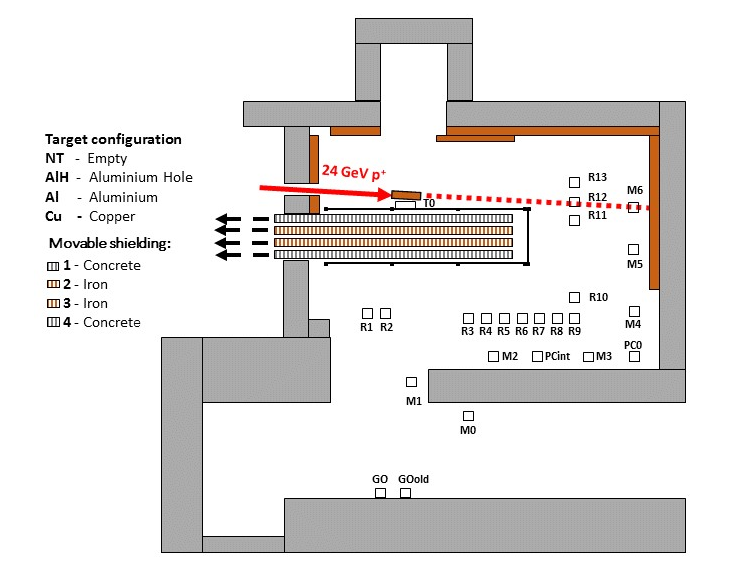
\includegraphics[width=0.9\textwidth]{02_RadiationEffectsOnElectronics/images/charm.png}
    \caption{The floor-plan layout of the CHARM irradiation test facility showcasing the available testing positions~\cite{cern_charm_website}.}
    \label{fig:charm-layout}
\end{figure}

\begin{figure}[H]
    \centering
    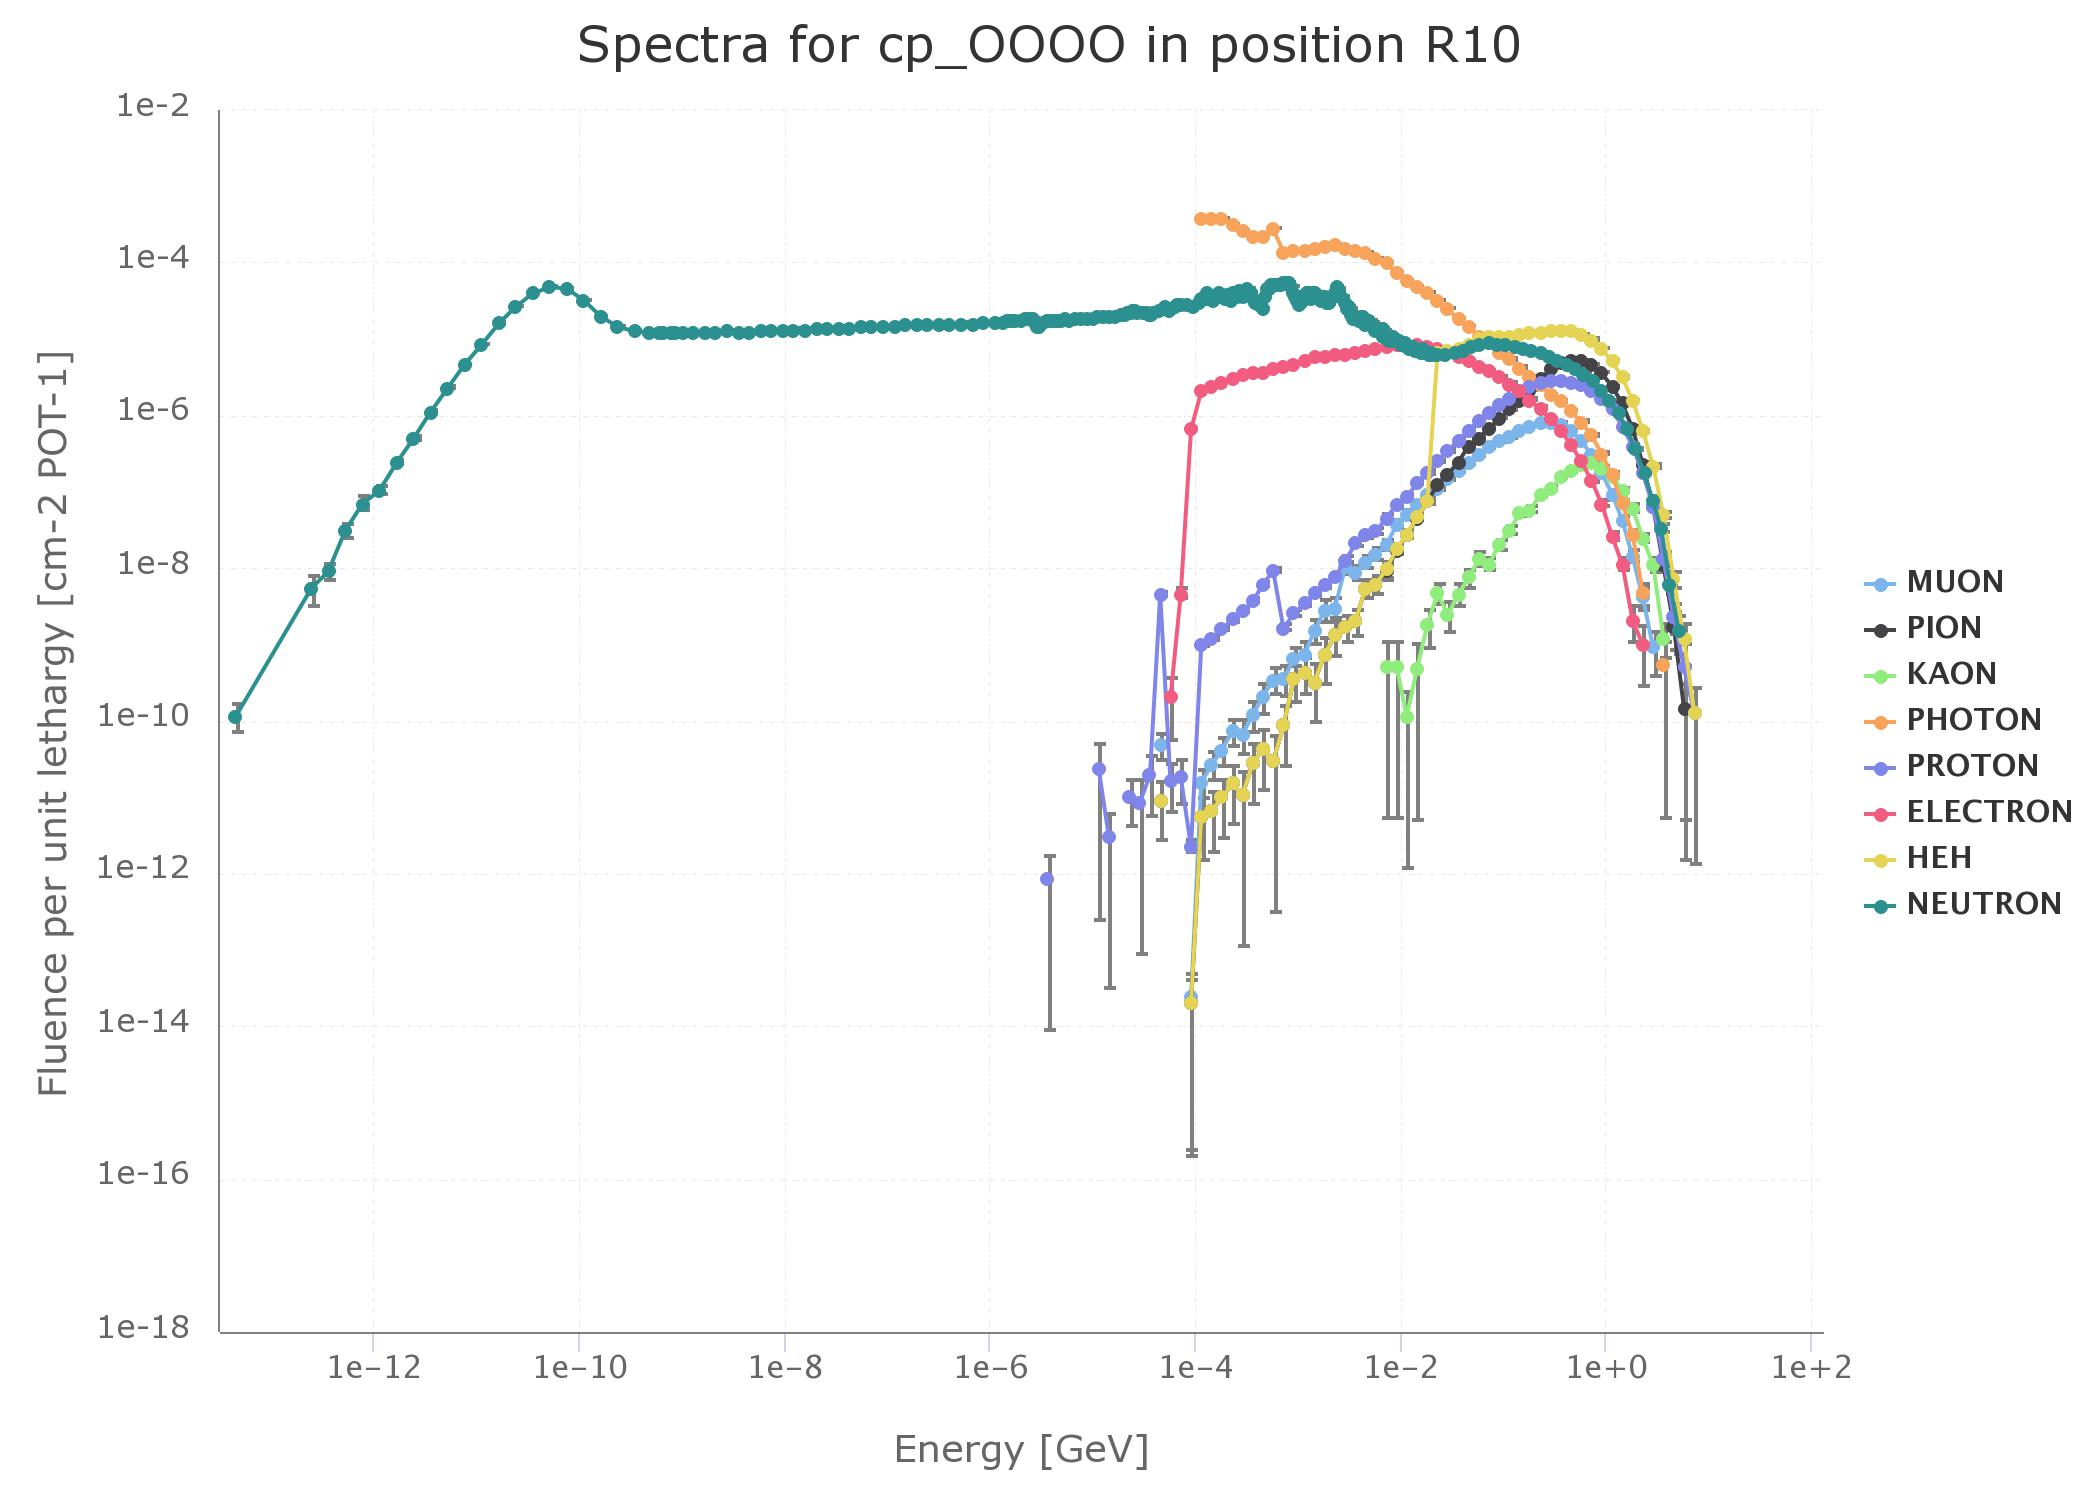
\includegraphics[width=0.9\textwidth]{02_RadiationEffectsOnElectronics/images/charm-particles-spectra.jpg}
    \caption{The particle spectra at the representative R10 testing position inside the CHARM facility~\cite{cern_charm_website}.}
    \label{fig:charm-spectra}
\end{figure}

\subsubsection*{CC60}
The CC60 facility, located at CERN, provides a $\gamma$-radiation beam utilizing a Cobalt-60 source. It offers several configurations to achieve different dose rates, which are adjusted by moving the table where the Device Under Test (DUT) is mounted closer to or further from the source. Tests performed at CC60 are ideal for evaluating system degradation under TID. Because the facility relies on typical photon irradiation, SEEs and DD—which are typically caused by high-energy hadrons—are not expected to occur.

\subsubsection*{Proton Irradiation Facility (PIF)}
The Proton Irradiation Facility (PIF) at the Paul Scherrer Institut (PSI) is located within the experimental area of the COMET cyclotron, which is primarily dedicated to proton therapy. The proton beam originates from the PROSCAN accelerator and undergoes primary energy degradation, delivering adjustable beam energies ranging from \qty{74}{\mega\electronvolt} to \qty{230}{\mega\electronvolt} to the PIF target area.

At PIF, the beam profile is relatively small, meaning the Device Under Test (DUT) should ideally fit within a standard \qtyproduct{50 x 50}{\milli\meter} aperture to ensure uniform exposure. Furthermore, the exceptionally high flux and dose rates achievable at this facility make it ideal for the rapid characterisation of component batches, avoiding the extended test campaigns—often spanning weeks—required at mixed-field facilities like CHARM.

However, it is worth noting that this proton beam is not fully representative of the complex LHC radiation environment. This is due to the absence of the complete mixed-field HEH spectrum resulting in a significantly lower DD-to-TID ratio compared to the actual operational conditions inside the LHC~\cite{ferraro_phd_thesis}.

\begin{figure}[H]
    \centering
    \begin{subfigure}[b]{0.48\textwidth}
        \centering
        \vfill
        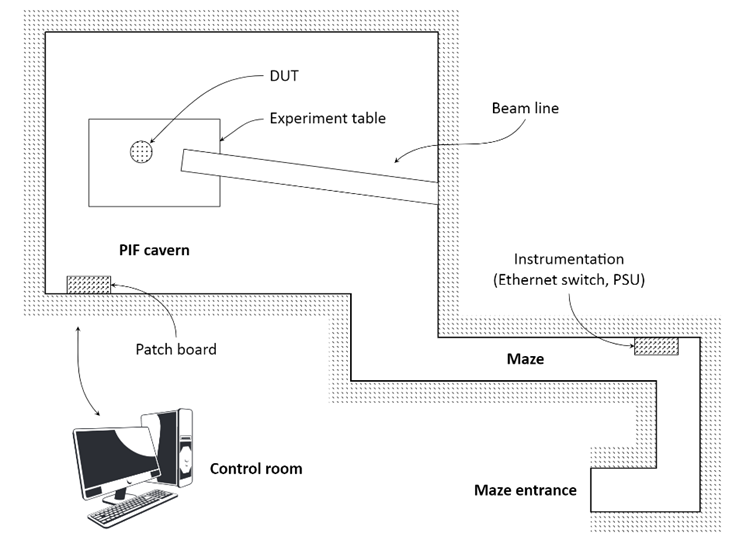
\includegraphics[width=\textwidth]{02_RadiationEffectsOnElectronics/images/psi.png}
        \caption{PSI layout}
        \label{fig:psi}
    \end{subfigure}
    \hfill
    \begin{subfigure}[b]{0.48\textwidth}
        \centering
        \vfill
        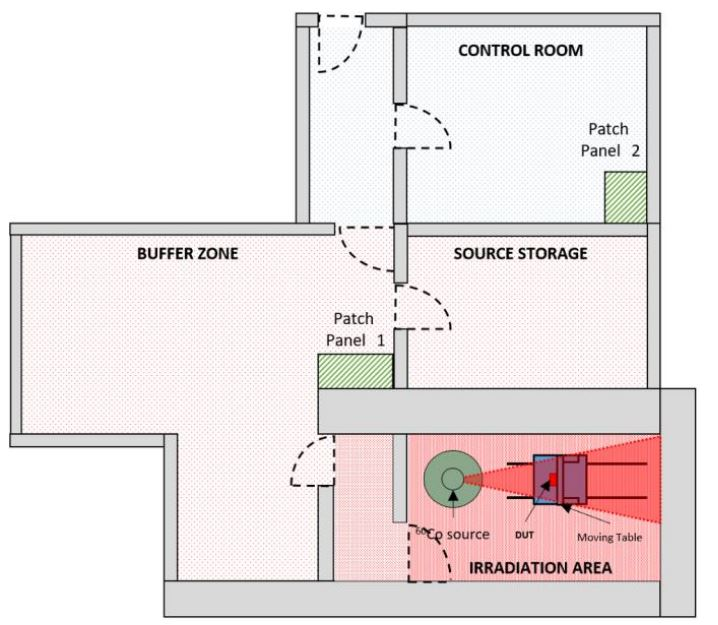
\includegraphics[width=\textwidth]{02_RadiationEffectsOnElectronics/images/cc60.JPG}
        \caption{CC60 layout}
        \label{fig:cc60}
    \end{subfigure}
    \caption{The floor-plans of the PSI and CC60 irradiation test facilities.}
    \label{fig:radiation-facilities-cc60-psi}
\end{figure}

\section{Effects of TID and DD on BJTs and MOSFETs}
\label{section:effects-bjt-mosfet}

\subsubsection*{Bipolar Junction Transistors (BJTs)}

Regarding degradation due to TID, it is mainly attributed to the increasing concentration of trapped charges at the $Si$/$SiO_2$ interface of the emitter-base junction, which leads to increased surface recombination and thereby to an increase in the base current $I_b$, and finally to degradation of the transistor's current gain. Furthermore, a leakage current across the collector-base junction is also expected due to inversion channel formation~\cite{ferraro_phd_thesis}.

Moreover, regarding DD, radiation creates defects in the silicon of the neutral base region and reduces the minority-carrier lifetime. Furthermore, this has consequences, as $I_b$ increases and the current gain changes. Both of these effects are linear and proportional to the particle fluence~\cite{ferraro_phd_thesis}.

One more thing that must be noted concerns the Enhanced Low Dose Rate Sensitivity effect (ELDRS), which is present in integrated bipolar circuits and makes their characterization much more complex at low dose rates.

In this thesis, bipolar technology will only be found inside integrated circuits, such as gate drivers~\cite{ferraro_phd_thesis}.

\begin{figure}[H]
\centering
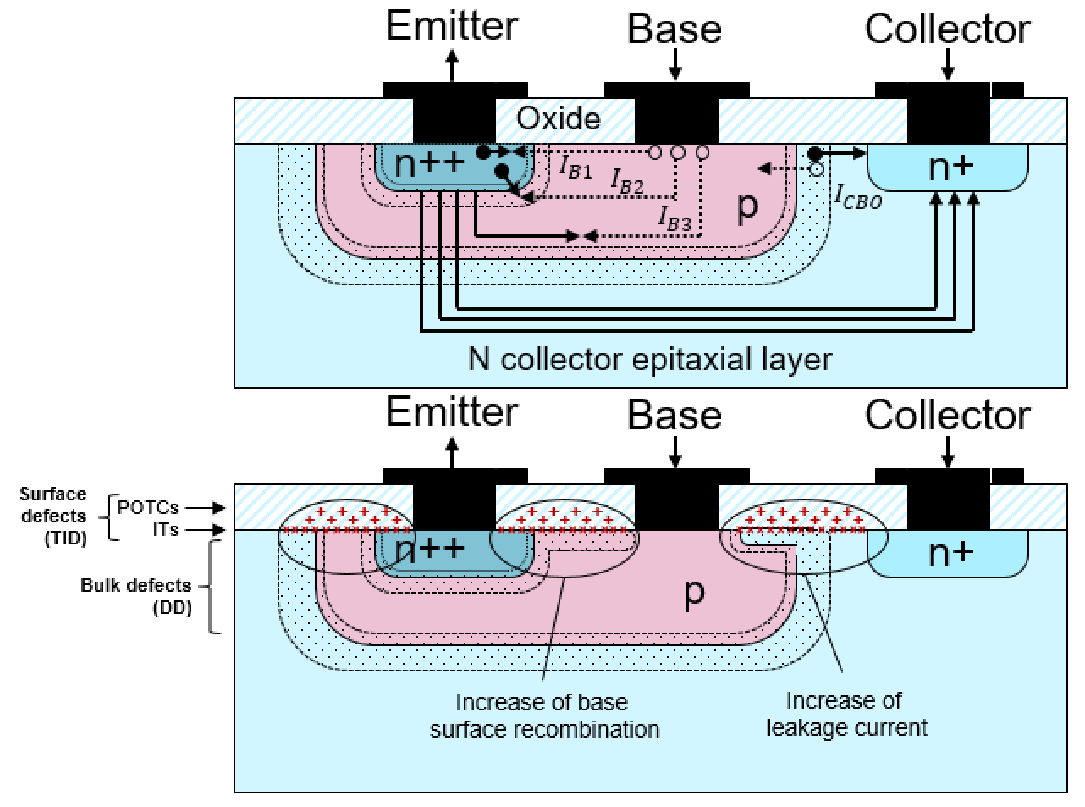
\includegraphics[width=0.9\textwidth]{02_RadiationEffectsOnElectronics/images/bjt-degradation-mechanism-2.png}
\caption{BJT degradation mechanisms due to TID-induced leakage currents and DD-induced lattice defects~\cite{ferraro_phd_thesis}.}
\label{fig:bjt-degradation-mechanism}
\end{figure}

\subsubsection*{Metal-Oxide-Semiconductor Field-Effect Transistors (MOSFETs)}

Firstly, as MOSFETs are, in principle, majority-carrier devices, they are extremely robust against the effects of displacement damage. However, they can still degrade due to TID. As with BJTs, both oxide- and interface-trapped charges can degrade the electrical parameters of MOSFETs. The main degradation factors, and the ones that circuit designers must be aware of, are \textit{i) the shift in $V_{gs}$} and \textit{ii) the increase in leakage currents}~\cite{ferraro_phd_thesis}.

While leakage currents mostly affect CMOS integrated devices, the shift in gate voltage is a greater concern for power MOSFETs. According to their working principle, when a sufficiently high gate-source voltage $V_{gs}$ is applied, minority carriers are attracted towards the substrate-oxide interface, and an inversion channel is created between the source and drain, thus allowing current to flow through it. Therefore, as the accumulation of trapped charges near the oxide and interface increases, the required voltage value changes and typically shifts towards negative values for NMOS devices. This can be visualized in Figure~\ref{fig:mosfet-degradation-mechanism}. Thus, for a circuit designer, the main concern is that the MOSFET may no longer be able to turn off after a certain dose~\cite{ferraro_phd_thesis}.

Finally, it should be noted that the degradation of MOSFETs, as opposed to that of BJTs, is not dependent on the dose rate~\cite{ferraro_phd_thesis}.

\begin{figure}[H]
\centering
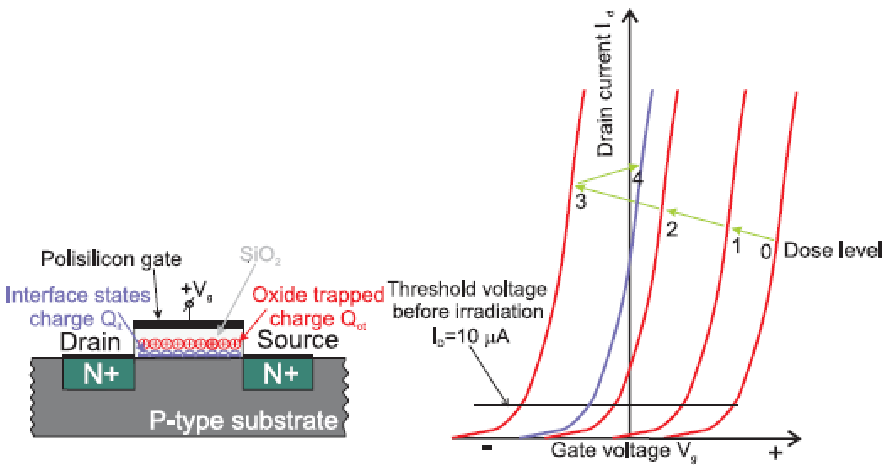
\includegraphics[width=0.9\textwidth]{02_RadiationEffectsOnElectronics/images/mosfet-degrdation-mechanism.png}
\caption{TID-induced shift of the MOSFET $V_{gs}$ characteristic curve~\cite{ferraro_phd_thesis}.}
\label{fig:mosfet-degradation-mechanism}
\end{figure}
